\chapter{Software design and structure}
With the theory of mazes and random number generation thoroughly briefed we can now explore the implementation of these algorithms. The software has a high level of abstraction and is designed to maximise code re-usability. It was developed in C++ and OpenGL; it is ported on both Mac OS X and Windows which further encourages code re-usability. Despite being implemented using OpenGL, the generator itself remains fully independent from OpenGL and can even be re-used with a different graphics library such as Microsoft's DirectX.

{\em DunGen} is the name of the software that was produced in parallel to the research. The software is designed as an extendible framework for dungeon generation. It implements most of the techniques discussed regarding maze and dungeon generation. It also contains a sample application in which a green wire-framed cube can be moved by the user and collide with the walls of the maze. All the source code is found in the {\em src} directory.

See appendix \ref{screenshots} for screen-shots of the final product and appendix \ref{codeDiagrams} for code listings and class diagrams

\section{The Engine}
The Generator is intended to be engine-independent. However, for the purpose of demonstration, a small engine was developed. The software runs using OpenGL and the math library GLM although it is possible to port the code to use other libraries. The engine used in the software is very primitive because it is only meant to be used to render the maze, handle axis-aligned bounding box (AABB) collisions and listen to user-input.

\paragraph{Features}
The features of the engine are found in the following directories:
\begin{itemize}
\item {\bf Engine/Core/Application/} Contains classes regarding argument-parsing and starting/exiting the application.
\item {\bf Engine/Core/File/} Used for handling files on different platforms.
\item {\bf Engine/Core/Timing/} Keeps track of timing in a static class.
\item {\bf Engine/Graphics/Camera/} The camera class containing values for {\em pitch}, {\em yaw}, {\em roll}, {\em field-of-view}, {\em near-clip-plane} and {\em far-clip-plane}.
\item {\bf Engine/Graphics/GraphicsContext/} Controls graphics context. GLFW is used to manage this on different platforms.
\item {\bf Engine/Graphics/Material/} Class describing the material of a 3D object.
\item {\bf Engine/Graphics/Mesh/} The Mesh class containing vertex positions, UVW co-ordinates and primitive indices.
\item {\bf Engine/Graphics/Renderer/} The class used to render the content of the scene.
\item {\bf Engine/Graphics/Texture/} Image bitmap handling, used by Mesh instances to diffuse a texture. The library SOIL is used to load PNG files.
\item {\bf Engine/Input/} Contains classes to examine keyboard and mouse states.
\item {\bf Engine/Scene/} Contains classes to control the content of the scene.
\item {\bf Engine/Tools/} Math functionalities.
\end{itemize}

\section{The Generator}

\subsection{The Maze}
The maze can be viewed as a static graph. It is composed of vertices (called cells) and edges (called walls); hence there are 3 classes used to represent the maze:
\begin{itemize}
\item \texttt{Maze}: The maze itself. It contains all the maze-cells and walls within an array. It also contains several queries and operations that can be used by a multitude of algorithms.
\item \texttt{MazeCell}: This class represents a single cell. It contains a {\em visited} field because this is essential for maze generators. It also contains its $x$ and $y$ co-ordinates to make it fast and simple to know where the cell is situated.
\item \texttt{MazeWall}: This class represents either a vertical or horizontal wall. It can be either of type 
\texttt{MAZE\_WALLTYPE\_NONE} (no wall) or \texttt{MAZE\_WALLTYPE\_DEFAULT} (there is a wall), this domain can easily be extended to support different types of walls, such as doors for instance.
\end{itemize}

\subsection{Graph Implementation}

There are multiple different structures that implement the graph data structure. Each one has its advantages and disadvantages. M. Goodrich and R. Tamassia have listed a number of possible suggestions in their book {\em  Data Structures And Algorithms in Java} \citep{DSAJ-4}.
\begin{itemize}
\item {\bf Adjacency List:} In this data structure, the vertices are stored in a linked list. Each vertex also stores a list of adjacent vertices. This structure is optimised for adding and removing edges or vertices very fast with a complexity of $\bigo{1}$ \citep{DSAJ-4}.
\item {\bf Incident List:} Very similar to the adjacency list structure, however incident rays are also stored in a list. Likewise, this structure is optimised for adding and removing elements of the graph \citep{DSAJ-4}.
\item {\bf Adjacency Matrix:} In this structure data of adjacent vertices is stored in a 2D array. This method is not very memory efficient for sparse graphs and is very slow at adding or removing vertices (complexity $\bigo{V^2}$). One big advantage though is that this structure has a complexity of $\bigo{1}$ for queries, making it ideal for static dense graphs \citep{DSAJ-4}.
\end{itemize}

In order to implement the maze, a data structure similar to that of the adjacency matrix was chosen. However the elements of the matrix store the vertices (cells) themselves and not the adjacent vertices. The reason for this is that the maze's dimension is completely static and the adjacent vertices are pre-defined. The dimension of the maze is only specified once at the initialisation and cells are never removed. In contrast to arrays, lists are optimised for dynamic structures that require frequent adding and removal, which is entirely unnecessary in this case and hence arrays are favourable \citep{DSAJ-4}. 

Arrays provide the advantage of direct access through the use of an index. This is exceptionally useful because cell query operations are very frequent in the algorithms that we have observed in the previous chapters. The cells are stored in a single dimensional array to keep memory contiguous but this array is used as a two-dimensional array. The 1D index of a cell $(x,y)$ in a 2D space can be calculated by the formula:
$$ I_{cell}(x,y) = x + yW \;\;\;\;\;\; \text{where }W=\text{width of the maze} $$

As mentioned previously, the incident edges do not need to be stored because given a cell $(x, y)$, we know that this cell has 4 adjacent nodes: $(x+1,y)$, $(x-1,y)$, $(x,y+1)$ and $(x,y-1)$ (assuming that $(x, y)$ isn't a borderline cell). However, data about the walls still needs to be stored somewhere. This is stored in an array for same reasons the that cells are. Vertical and horizontal walls are stored in separate arrays; the reason for this is the two arrays are of different dimensions. In mathematical terms
\begin{itemize}
\item Let $W=$ the number of cells along the $x$-axis.
\item Let $L=$ the number of cells along the $y$-axis.
\item The dimension of the vertical wall array is $(W+1,L)$.
\item The dimension of the horizontal wall array is $(W,L+1)$.
\end{itemize}

\subsection{Random Number Implementation}
All the algorithms have some kind of randomness within them. The randomness in these algorithms remains abstract and changing the behaviour of how random elements are chosen can effect the outcome of the dungeon, much like how the Growing Tree algorithm can generate different types of mazes based on how the random selection works \citep{ThinkLabyrinth}.

Concerning random number generation in PCG something simple such as a LCG will suffice. LCGs are not cryptographically secure but this is not an issue because there is no need to hide anything. Additionally LCGs provide the advantage of being fast and reproducible. So if we do not want to store a generated dungeon because of memory concerns then we can simply store the seed and run the algorithm again to restore the old dungeon. Needless to say, research has shown that we need good parameters to obtain numbers that are statistically adequate. Finding a good LCG is a difficult task, so instead we will simply use the one suggested by Park and Miller because that one has a large amount of evidence supporting its reliability. Reminder: The coefficients of this LCG are $M = 2^{31}-1$, $a = 7^5$ and $c = 0$. Normally on the lower-order bits would have to left un-used because they produce bad results, however this is not necessary in this case because the modulus in not of the form $2^i$ \citep{park_miller}.

For the most part, we can simply used an integer generator with a uniform distribution. Random elements can be picked from a set by generating a random index within range. However in some cases we might need a non-uniform distribution. For instance, let us consider the DFS maze generation algorithm. If a uniform number generator is used then the algorithm will have an equal chance to turn right, to turn left or carry on straight. This means that the probability of carrying on straight is $\frac{1}{3}$ and the probability of turning is $\frac{2}{3}$ (assuming that all 3 options are available), which will trivially cause lots of turns to occur. If we want to reduce this we can use the class {\tt RandomTurner} in the framework. This class uses a random-float generator to produce integers such that the probabilities of turning left, right or going straight are different. This is useful if we want to use a DFS or Hunt-And-Kill generator that turns less often.

The number generators can be found in the {\em Generator/Random/} directory. It consists of 2 interfaces:

\begin{enumerate}
\item {\bf RandomI:} This interface defines a random {\em Integer} generator.
\item {\bf RandomF:} This interface defines a random {\em Floating-point} generator.
\end{enumerate}

There is 1 class implementing both of these interfaces and 1 implementing only the \texttt{RandomI} interface. Respectively, these classes are:
\begin{enumerate}
\item {\bf UniformRandom:} This class produces random integers and floats that follow a uniform distribution. It uses a 32-bit LCG to produce these numbers.
\item {\bf RandomTurner:} This class is used by maze generators such as the depth-first search generator to allow more control over the probability of turning. It produces random integers between 0 and 2 using a \texttt{UniformRandom} instance and given probabilities.
\end{enumerate}

\subsection{Diggers}
At this stage, the dungeon generation algorithm is divided into a sequence of phases. Generating a dungeon consists of generating a maze and then applying some post-processing actions on it \citep{JBuck}:
\begin{enumerate}
\item Generate a maze.
\item Reduce density of maze.
\item Add loops in the maze.
\item Add rooms in the maze.
\end{enumerate}
\begin{figure}[h!]
\centering
 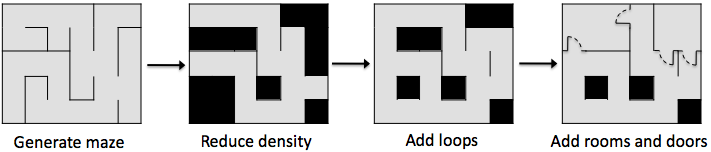
\includegraphics[width=0.66\textwidth]{images/makeDungeon4steps.png}
\caption{The 4 major steps to generate a dungeon.}
\end{figure}

If we interchange, remove or modify these phases we will obtain different result. Ideally, to keep the framework as generic as possible, the user should have full access to any of these phases and should be allowed to use them in whichever order they please to. To allow this kind of freedom to the user the DunGen framework will be based around these phases. Each phase will be referred to as a {\em Digger} and will alter the shape of the maze in some way.

All the diggers in the application extend the abstract \texttt{Digger} class that contains the initialisation, iteration and ending steps of the algorithm. Each digger implements the \texttt{Step} function (along with other functions) that corresponds to a single step in the algorithm. This function returns \texttt{true} once the looping is complete. To run a digger we need only to call the \texttt{DigFully} function that runs all these steps.
\lstCpp
\begin{lstlisting}
void Digger::DigFully()
{
	Init();
	while(!Step());
	End();
}
\end{lstlisting}

\paragraph{DFSDigger} This digger generates a maze using the DFS algorithm. The algorithm is implemented using a back-tracking stack\footnote{Actually a \texttt{std::list} is used, but it is used as a stack}. Every-time the algorithm visits a new node with more than one child it adds this node to the stack. Whenever it visits a new node with no children it backtracks by popping a node from the stack and carries on from there.
\paragraph{PrimDigger} This digger generates a maze using Prim's maze generation algorithm. It is implemented in a similar way to the Depth-first search digger, except that it uses a list instead of using a stack. The algorithm always adds newly visited nodes to the list and removes them when they no longer have any unvisited children. At the start of each iteration, a random node from this list is chosen.
\paragraph{KruskalDigger} Another digger used to generate a maze using Kruskal's algorithm. The algorithm is implemented with the use of the helper classes \texttt {KruskalEdge} and \texttt{SpanningTree} to quickly identify whether or not 2 cells belong to the same spanning tree.
\paragraph{BinaryTreeDigger} This digger generates a maze using the binary-tree maze generation algorithm. This digger simply removes either the top or left wall for each cell in the maze. However, it insures not to remove any walls at the extreme edges of the maze.
\paragraph{StartEndDigger} This digger simply creates a small 2x2 room on the top-left and bottom-right corners. This digger can be placed before the \texttt{DeadEndDigger} to prevent that digger from leaving the player in a 1x1 room.
\paragraph{DeadEndDigger} This digger increases the sparseness factor of a maze by walling off dead-ends. The {\em sparseness} factor defines the number of iterations to perform. On each iteration the digger finds all the dead-ends in the maze and walls them off.
\paragraph{LoopDigger} This digger uses a random float generator and a given probability to determine which dead-ends should be turned into loops. It uses a randomized walk similar to that in Wilson's algorithm \citep{DBLP:conf/stoc/Wilson96}.
\paragraph{RoomDigger} This digger places random rooms at any random positions in the dungeon. It simply breaks walls at random areas and doesn't check for any constraints.
\paragraph{WeighedRoomDigger} This digger, like the \texttt{RoomDigger}, also places random rooms across the dungeon. However, this digger uses a weighing system to find the best suitable way to place the rooms \citep{JBuck}.
\paragraph{WallDecoDigger} This digger randomly places external 3D meshes onto the walls. It provides file-names, translation and rotation that can be used by the engine to load the meshes.
\paragraph{DoorDecoDigger} Identical to the \texttt{WallDecoDigger}, but for the doors.

\section{Launcher}
The DunGen software comes with a Launcher developed in Java. This Launcher is designed to make it easy to quickly parametrise the dungeon generator and launch it. The Launcher is very useful to analyse how the dungeons created vary according to the parameters used. Number generators and diggers can be added, removed and configured as the user wants. The properties of the number generators and diggers are exported by the Launcher into a {\em .dungenprofile} file that is read by the DunGen program.

The user can specify which texture files to use to display the dungeon along with the random seed and maze dimension. Minimal graphics options are also available to the user. The launcher runs the DunGen program as a child process and displays the program output stream in a text-area.

All the source code of the DunGen launcher can be found in the {\em Projects/eclipse/Launcher/src/} directory. See appendix for screen-shots.

\begin{figure}[h!]
\centering
 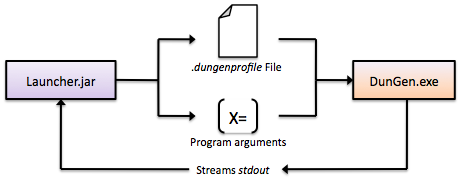
\includegraphics[width=0.52\textwidth]{images/launcherAndDungen.png}
\caption{Interaction between the Launcher and the DunGen program.}
\end{figure}